%%
%% This is file `sample-sigchi.tex',
%% generated with the docstrip utility.
%%
%% The original source files were:
%%
%% samples.dtx  (with options: `sigchi')
%% 
%% IMPORTANT NOTICE:
%% 
%% For the copyright see the source file.
%% 
%% Any modified versions of this file must be renamed
%% with new filenames distinct from sample-sigchi.tex.
%% 
%% For distribution of the original source see the terms
%% for copying and modification in the file samples.dtx.
%% 
%% This generated file may be distributed as long as the
%% original source files, as listed above, are part of the
%% same distribution. (The sources need not necessarily be
%% in the same archive or directory.)
%%
%% The first command in your LaTeX source must be the \documentclass command.
\documentclass[sigchi]{acmart}
\usepackage{csquotes} 

%%
%% \BibTeX command to typeset BibTeX logo in the docs
\AtBeginDocument{%
  \providecommand\BibTeX{{%
    \normalfont B\kern-0.5em{\scshape i\kern-0.25em b}\kern-0.8em\TeX}}}

%% Rights management information.  This information is sent to you
%% when you complete the rights form.  These commands have SAMPLE
%% values in them; it is your responsibility as an author to replace
%% the commands and values with those provided to you when you
%% complete the rights form.
\setcopyright{acmcopyright}
\copyrightyear{2020}
\acmYear{2020}

%% These commands are for a PROCEEDINGS abstract or paper.
% These commands are for a PROCEEDINGS abstract or paper.
\acmConference[JCDL, 2020]{JCDL '20: Joint Conference on Digital Libraries}{June 19-23, 2020}{Wuhan, Hubei, P. R. China}
\acmBooktitle{JCDL '20: Joint Conference on Digital Libraries, June 19-23, 2020, Wuhan, Hubei, P. R. China}
\acmPrice{}
\acmDOI{}
\acmISBN{}

%%
%% Submission ID.
%% Use this when submitting an article to a sponsored event. You'll
%% receive a unique submission ID from the organizers
%% of the event, and this ID should be used as the parameter to this command.
%%\acmSubmissionID{123-A56-BU3}

%%
%% The majority of ACM publications use numbered citations and
%% references.  The command \citestyle{authoryear} switches to the
%% "author year" style.
%%
%% If you are preparing content for an event
%% sponsored by ACM SIGGRAPH, you must use the "author year" style of
%% citations and references.
%% Uncommenting
%% the next command will enable that style.
%%\citestyle{acmauthoryear}

%%
%% end of the preamble, start of the body of the document source.
\begin{document}

%%
%% The "title" command has an optional parameter,
%% allowing the author to define a "short title" to be used in page headers.
\title{Seeking Justification: How Expert Reviewers Validate Empirical Claims with Data Annotations
}

%%
%% The "author" command and its associated commands are used to define
%% the authors and their affiliations.
%% Of note is the shared affiliation of the first two authors, and the
%% "authornote" and "authornotemark" commands
%% used to denote shared contribution to the research.
\author{Nicholas Weber}
\email{nmweber@uw.edu}
\affiliation{%
  \institution{University of Washington}
  \city{Seattle}
  \state{WA}
}

\author{Sebastian Karcher}
\email{skarcher@syr.edu}
\affiliation{%
  \institution{Qualitative Data Repository, Syracuse University}
  \city{Syracuse}
  \state{NY}
}



%%
%% By default, the full list of authors will be used in the page
%% headers. Often, this list is too long, and will overlap
%% other information printed in the page headers. This command allows
%% the author to define a more concise list
%% of authors' names for this purpose.
\renewcommand{\shortauthors}{Removed}

%%
%% The abstract is a short summary of the work to be presented in the
%% article.
\begin{abstract}
We investigate the use of data annotations to increase transparency and data access in social science research. We present preliminary findings from a study that asked experts to review a research paper and judge the validity of empirical claims made - first without data and then with annotations that provide access to underlying data. We demonstrate that in domains where there is an emergent culture of data sharing reviewer expectations about what material should be shared are met, but this does not necessarily influence trust in an author's claims. Reviewers describe ways that shared materials aide validation tasks, but that these materials just as often sharpen their critique and introduce new lines of questioning. We believe that these findings hold important implications for scholarly communications and digital repository development, in particular as these two communities engage in developing policies to guide authors on how to prepare data for review, supporting reviewers with linked repository systems, and for the design of peer-review processes more generally. 
\end{abstract}

%
% The code below is generated by the tool at http://dl.acm.org/ccs.cfm.
% Please copy and paste the code instead of the example below.
%
\begin{CCSXML}
<ccs2012>
<concept>
<concept_id>10002951.10003227.10003392</concept_id>
<concept_desc>Information systems~Digital libraries and archives</concept_desc>
<concept_significance>500</concept_significance>
</concept>
</ccs2012>
\end{CCSXML}
\ccsdesc[500]{Information systems~Digital libraries and archives}
%
%% Keywords. The author(s) should pick words that accurately describe
%% the work being presented. Separate the keywords with commas.
\keywords{Scholarly Communications, Annotations, Open Data, Transparency, Peer Review}


%%
%% This command processes the author and affiliation and title
%% information and builds the first part of the formatted document.
\maketitle

\section{Introduction}
Transparency is a fundamental norm in scientific practice \cite{merton1942science}.  Research findings are based not solely on trust, but the ability for peers to access and review the logic behind how data were interpreted and claims were made using sound reasoning \cite{pedersen_empiricism_2008}. The Royal Society for Science Policy states this succinctly, “...science communication is assessable communication, which allows those who follow it not only to understand what is claimed, but also to assess the reasoning and evidence behind the claim” \cite{royal_society_great_britain_science_2012}. Many scientific domains have become dependent upon large stores of data, software, and computing resources that add new layers of complexity to both producing and communicating research findings. This in turn has motivated new transparency initiatives by scholarly societies, national funding agencies, and academic publishers. Depending on the type of research that is being produced transparency can be promoted in pursuit of reproducibility or replication \cite{open2012open}; validation \cite{fischer2019politics}; or even ethical reporting of results \cite{nicholls2016reporting}. 

What unites different trends in research transparency is a call for greater access to the underlying materials used to produce an empirical finding: data, research instruments, and  software are all expected to be shared in a research ecosystem that is as ‘open as possible, but as protected as necessary’ \cite{wilkinson2016fair}. In the following paper we present preliminary findings from a research project that investigates the impact of increased research transparency on the evaluation of an empirical claim outside of a formal peer review process. Our investigation is specifically focused on qualitative and mixed methods research where there has been considerably less infrastructural support for archiving, sharing, and reusing data \cite{elman2014data}. We investigate how and in what ways experts use  data in their peer review assessment, and the potential impact that data annotations have on their ability to establish trust in claims made within a scholarly article. The sections that follow describe the background setting, our study methodology,  findings of two separate data collection events, and the implications of this work for developing policies to guide authors on how to prepare data for review.

\section{Background} 
A number of previous studies have focused on how researchers comply with different mandates for practicing open science, including adherence to expectations of transparency in publication \cite{tong2012enhancing}, data sharing \cite{peat2014improving}  and ethical statements about research conduct \cite{anderson2013ethical}. Although these studies have provided a valuable basis for evaluating the efficacy of open science policies, there has been considerably less attention paid to the downstream impacts that these initiatives may have on the evaluation of research outputs. For example, we know relatively little about how data sharing policies enforced by journal editors might be used in reviewing a manuscript for publication, or how program officers use data management plans to evaluate the outcomes of a funded research grant. In this study, we are particularly interested in better understanding how increased access to data impacts peer evaluation and claim acceptance. 

Central to the task of peer review is a validation process where experts are asked to judge a claim based on available evidence \cite{spier2002history}. As a critical component of transparency initiatives, scholarly journals have been encouraged to develop data sharing requirements \cite{schofield2009post, sturges2015research} that require authors to provide underlying data along with manuscript submitted for review. The logic of this policy advocacy is that by intervening in a process of research dissemination scholarly publishers can play an important role in assuring that research results are valid and replicable . However, empirical studies from both the life sciences \cite{vasilevsky2017reproducible,thelwall2017journal}, and social sciences \cite{crosas_data_2018} have demonstrated that data sharing policies are not universally adopted nor enforced. 

Previous research has also shown that shared data increase increase the possible reproducibility of published findings in the natural sciences \cite{vanpaemel_are_2015, hardwicke_data_2018}. By and large, these studies are limited to quantitative analysis that include simple statistical checks for robustness. Outside of computational reproducibility, there has been little research into how shared data are used to validate claims or how shared data impact trust in findings. Even the policy motivations for transparency often gloss over the peer review process and instead focus on the need to either cite data or share resources in order to increase the efficiency of reusing materials to further new research \cite{parsons_data_2010}.    

Previous studies have also demonstrated a positive correlation between openly shared data and citations (a so called open data advantage \cite{piwowar_sharing_2007, christensen_study_2019}). Publishers see the open data advantage as a motivation for drawing attention to their journals. However, we argue that without understanding how new requirements for sharing data, instruments, and software impact the trust that reviewers have in a research finding the scholarly communications ecosystem still faces a dilemma in knowing what types of resources, in which forms, and through what modes of access are valuable. 

We recognize that understanding how reviewers make sense of, use, and seek data in validating an empirical claim during peer review remains challenging \cite{kratz_researcher_2015}, and for good reasons: It is difficult to disentangle which policies are promoted by which journals and under what circumstances policy compliance is regulated \cite{crosas_data_2018}. Further, it is difficult to  study peer review without, unintentionally, disrupting an already burdensome validation task that often goes unrewarded. But, calls for greater understanding of peer review processes are decades old with relatively little progress made in the intervening years \cite{bailar_journal_1985, lee_promote_2017}. In the following study, we seek to better understand how it is that reviewers interpret and use shared data through an initiative - Annotation for Transparent Inquiry - that focuses on using open web annotations to increase the transparency of a research claim.\\ 
\subsection{Annotation for Transparent Inquiry}

Annotation for Transparent Inquiry (ATI) was developed by the Qualitative Data Repository (QDR) and supported by research grants from the National Science Foundation (NSF) and Robert Wood Johnson Foundation (RWJF) \cite{elman2018qualitative}. ATI builds upon a tradition in qualitative research that encourages three forms of transparency: 
\begin{itemize}
    \item \textbf{Data}: The evidence used to produce a research claim are made accessible. 
    \item \textbf{Analytic}: The processes for analyzing data are explained and made clear, including how evidence was used to advance descriptive, interpretive, or causal claims. 
    \item \textbf{Production}: The selection of appropriate methods, evidence, and arguments are justified, and situated amongst possible choices \cite{moravcsik2014transparency}  
\end{itemize}
ATI is an attempt to enable qualitative and mixed-methods researchers to more easily deploy each of these three forms of research transparency through the use of open web-annotations \cite{karcher2019annotation}. In producing an empirical manuscript, a researcher is encouraged to provide data, analytic, and production annotations so that readers and reviewers might more easily interpret and evaluate their work. In the ATI example pictured below (taken from \cite{omahoney_data_2019}), annotations provide \textit{data access} by linking to a digitized copy of the cited primary source; it provides \textit{analytic transparency} by clarifying which part of the source supports the claim in the text (via the source excerpt) and how it does so (as part of the analytic note); and finally it provides  \textit{production transparency} by explaining the exact provenance and context of the excerpt.

\begin{figure*}[tb]
\centering
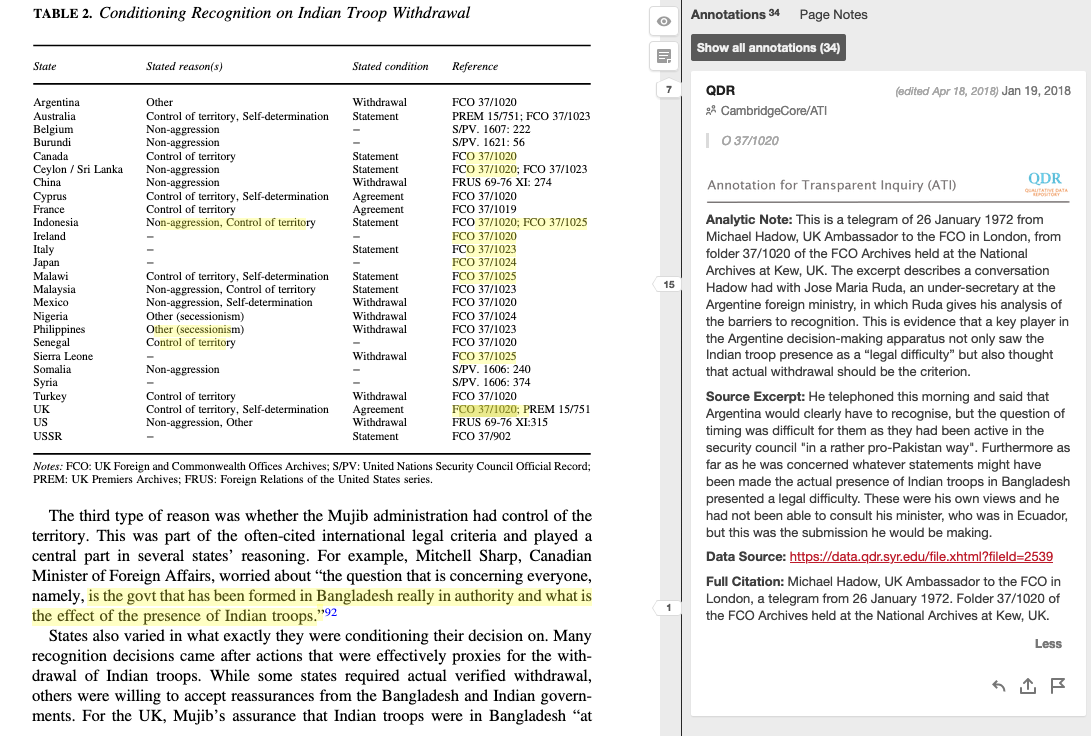
\includegraphics[width=\textwidth]{ATI.png}
\caption{An example of an ATI project where the author has annotated a table reference, provided a link to the source, and an explanation of the choice for its inclusion.}
\end{figure*}

\section{Methodology}
Our study of transparency in qualitative and mixed methods research took place in two separate data collection events. We recruited two sets of authors and reviewers to participate in each study using annotated publications and shared data. The design of the study is meant to answer the research question: \textit{How do data annotations impact the evaluation of empirical research by expert peer-reviewers?} Based on previous research \cite{kratz_researcher_2015,morey_peer_2015,nicholls2016reporting}, we hypothesize there will be three effects: 
\begin{itemize}
\item \textbf{H1:} Data annotations will improve reviewer’s access to underlying source materials when reviewing an article.
\item \textbf{H2:} Data annotations will improve the ability of a reviewer to validate an empirical claim. 
\item \textbf{H3:} Data annotations will improve the trust reviewers have in an author’s overall argument. 
\end{itemize}

To test these hypotheses we first purposefully recruited a two sets of authors that had published, or were in the process of publishing, an article using qualitative or mixed methods. The first set of authors had already published a manuscript and the second set of authors were in the process of either publishing or completing a first draft of their article for submission to a peer-reviewed journal. To qualify for the study the author's articles had to contain an empirical claims that could be elucidated by or improved with an annotation that connected a primary source (data) or logic of analysis to a research finding. Both sets of authors were recruited by email and enrolled after having agreed to annotate their articles following directions provided by our research team (n=35 total for both sets of authors). Authors were instructed to create annotations that focused on improving the transparency of their article by adding necessary contextual information, analytic notes, or attaching data to places in the text where a claim was made (e.g. data, analytic, or production transparency). After author annotations were complete our research team then assembled the data that authors provided and published their paper, annotations, and data to a password protected web repository. Annotations created by the author were then anchored to web documents using the open-source software Hypothesis [https://web.hypothes.is]. 

We then recruited a set of expert peer reviewers (n = 34 total) to judge the efficacy of the authors' annotations for improving transparency. Reviewers were recruited by our research team, and through suggestions from authors who identified experts in their field. Reviewers were first instructed to read an author’s article, published on the web, without annotations. They were to record in a pre-test logbook sections of the paper where not enough evidence was offered to validate a claim, and to document where they expected additional explanations or data to be provided by the author through annotation. Reviewers were then given the author’s annotated article and, in some cases, access to password protected repository containing the author’s original data. Reviewers re-read the author’s publication with annotations and supplemental data. Reviewers then recorded in a post-test logbook whether or not their expectations had been met. 

We collected both the pre- and post-test logbooks from reviewers, and analyzed their responses using the qualitative analysis software Dedoose. We used thematic analysis \cite{braun2006using} to identify patterned responses from the reviewer logbooks that fit one of our three stated hypothesis. To do so, our research team first developed a codebook to describe the contents of reviewer logbooks. We first coded five of the same reviewer logbooks. We noted places in the pre- and post-test logbooks that addressed our three hypotheses (stated above) and the relation to themes implied by each hypothesis (trust, validation, and access). We then compared our codes for similarity, discussed the definition of each code, and arrived at a set of definitions that would be used to analyze the rest of the logbooks. The lead author then coded the rest of the logbooks to identify the three themes (trust, validation, and access). After completing coding of all data we aggregated responses in relation to each stated hypothesis, discussed relevant quotes, and the representativeness of reviewers comments. In the following sections we present findings from reviewers based on their evaluation of an article using data annotations. 

\subsection{Results}
Reviewers responded to annotations in service of strengthening claims, improving access to underlying materials, and deepening trust. We discuss these topics in the context of our stated hypotheses below. Where possible we provide direct quotes and interpretations from reviewers. To attribute quotations of reviewers in this article we provide in brackets the reviewer ID used by our research team during analysis. These simple numerical identifiers are anonymous and do not allow for reidentification of our participants.\\ 

\textit{H1: Data annotations will improve reviewer’s access to underlying source materials when reviewing an article}\\

From the post-test logbooks reviewers reported that annotations improved their access to supporting materials during review. In many instances, providing data through linked annotations allowed reviewers access that would not have been otherwise possible. As one reviewer noted, “By providing quotes and links to images/scans, the author made accessible sources I’d otherwise have to either ask them for privately, or recover myself in London.” [R-1]  This reviewer went on to describe the value of having immediate access to rare historical and archival documents that they would have not been able to reliably identify with citation information alone. 

Annotations provided more immediate access to research materials and improved data transparency, but analytic and production transparency (described above) was more difficult to achieve. In particular, some reviewers found it difficult to disentangle access and trust. This was clear when being given access to underlying materials in service of a claim changed their expectations of what the original article could have achieved without shared data, 

\begin{displayquote}
“The annotations certainly made the claims more trustworthy, although I am not sure that is the best word for how they supported the arguments within the text. Rather, I would say that being able to access the original survey and interview instruments revealed the ‘backstage’ of the research production, and helped me reconstruct the process the researchers followed from observation to research findings.” [R-1] 
\end{displayquote}
The ability to go "backstage" as this reviewer notes, was seen as a way to better connect how data were related to both analytic and production transparency. Another reviewer similarly noted that “The source quotes and analytic notes were usually sufficient to understand and strengthen the point being made. But the mere fact of having access to the original sources did bolster my confidence in the claims being made.” [R-2] What these two reviewers make clear is that ease in access to underlying data both improves confidence in the authors work overall, but allows them to focus on and extend a form of trust to their empirical claims. We return to this relationship between our hypothesis related to access and trust in the discussion section below.  

For articles that included a mixed methods component, using both qualitative and quantitative analysis, increased access was seen as providing greater robustness. One reviewer of a mixed-methods linguistic article noted this in saying the following, 
\begin{displayquote}
“I fully interacted with the data sources provided by the authors: the sound files, transcripts, transcription guidelines and screenshots of the statistical models. I found they provided me with a fuller understanding of the dialect and its nuance...the mere presence of the sources was something of a stamp of approval, an extra layer of robustness to the piece I was reading.” [R-3]
\end{displayquote}
In this particular paper the authors had provided sound files that allowed for the linguistic phenomena to be heard by the reader throughout the article. This is a unique example of data transparency in that annotations afforded not just access to the data, but convenient ways of presenting the data to readers. By allowing the reviewer to stay within the article and listen to the speech excerpts the reviewers attention remained focused on the phenomena of interest rather than the practicalities of locating and accessing shared data. We believe this is an important affordance of using annotations for data transparency - ease of access reduces reviewer fatigue in context switching (between text and data) and thus allows for concentrated attention on arguments being advanced, and claims being made. 

The broad consensus of reviewers, through our analysis of pre- and post-test logbooks, confirmed the first stated hypothesis: Data annotations improved reviewer’s access to underlying source materials when reviewing an article with empirical claims.\\ 

\textit{H2: Data annotations will improve the ability of a reviewer to validate an empirical claim.}\\

Next, we examine the effect of annotations on reviewers when attempting to validate an empirical claim. As \citet[45-46]{elman2014data} point out, evaluating qualitative research and validating its empirical claims requires all three forms of transparency. Evaluating entails assessing "whether the authors’ data-generation techniques were aligned with the rules of inference and interpretation they were following" (production). It entails (among other things) "assessing the micro-connections between individual pieces of (cited) data and descriptive/causal inferences or interpretation". And in many cases it will require access to the data, for example in order to assess "how authors drew observations from sources, for instance, reading their interview transcripts to assess whether they asked leading questions or in some other way biased their interviews." \cite{elman2014data}

From our analysis of pre- and post-test logbooks, there was no broad consensus in reviewers comments on whether or not annotations were effective for claim validation. Reviewers that did not find annotations helpful noted a gap between their expectations of authors, given extended time and capability for clarifying their claims, and what was actually supplied with data annotations. As an example, one reviewer’s pre-test logbooks stated that they had four expectations for annotations regarding the claims made in an article that drew upon observational and interview data. But, these were not the passages that the author choose to actually annotate. This reviewer responded to this gap by saying, “Most of the annotations were about the factual claims about the context of the study, rather than about the main arguments of the paper.” [R-5]. Another reviewer similarly notes, 

\begin{displayquote}"In many of the sentences and sources I flagged, I suggested that excerpts and summaries of the source points would strengthen interpretations...I think providing excerpts and summarizing how the sources supported the given sentence would have further strengthened the article and made it more tractable for readers in some points, but were not necessary to correct deficits." [R-11]\end{displayquote} 

In these example, the reviewers draw attention to the various roles that data annotation can play. In some instances claims were indeed easier to interrogate with data annotations, but reviewers also noted that authors tended to use annotations for easy to substantiate facts rather than to add additional support for a research claim. In other words, authors tended to use annotations in service of data transparency by explaining how factual information were linked to an advanced claim, but authors failed to fully utilize annotations for production and analytic transparency that would have explained why this data was relevant evidence for a stated finding. 

Reviewers also reported that they could not validate a claim because data were supplied without enough context for accurate interpretation. A reviewer of a medical anthropology article describes this as follows, 
\begin{displayquote}
"Some of the background claims about the scarcity of livers could not be supported very well because of a lack of data available for the UK and a report that was unavailable. The claims about the risks particular to split liver transplants could have been better supported with further annotations and references. Some of the claims I felt were not well supported with the references." [R-20]
\end{displayquote}
In scenarios where data transparency was the barrier to claim validation reviewers often had unmet expectations between their pre and post-test logbooks. This importantly shows a gap in expectations about not only what data could have been provided, but also how that data should have been attached to textual claims to ease interpretation. This particular point of contention - between possibility and reality - speaks to a potential limitation in our study design; By asking reviewers to focus in particular on data and resource access they may have been primed to focus in particular on these aspects of an author's manuscript. Reviewer expectations in the context of this study should thus be read as idealistic with respect to transparency. That is, given time and technological assistance to provide as much transparency as possible, reviewers are evaluating an author's claims with heightened awareness of what is possible rather than what is normative. This relationship between potential transparency and normative expectations is thus challenged when introducing a new mode of scholarly communication like annotations. 

Overall, we do not find strong support for our second hypothesis. Reviewers felt that data annotations were helpful in interpreting a research result, but did not find the annotations helped them validate a claim explicitly. We return to this result in our concluding section.\\ 

\textit{H3: Data annotations will improve the trust reviewers have in an author’s overall argument.}\\

Similar to claim validation, reviewers did not reach consensus on whether or not their trust in an article was improved through annotations. Reviewers not reporting an increased trust dismissed the idea that they approach reviewing empirical work with a skepticism that would require an annotation or justification through shared data. A comparative political scientist that participated in the study explained their interpretation as follows, \begin{displayquote}
"I do not as a rule doubt mistrust my peers. But if I did, providing a full quote and link to a photo or scan of the original document cited would certainly offer an unimpeachable reference… The annotations did make it clear how the author was using archival documents to support their claims, but as this is a very simple and common method in qualitative research on historical cases, I did not really have any questions about this." [R-6] 
\end{displayquote}
This particular reviewer exemplifies an important distinction in participants of our study: Review and evaluation is very much related the epistemic commitments of a particular discipline or domain of research. As such, assumptions about the form and content of transparency annotations will necessarily differ between reviewers. Qualitative scholars that use archival materials often assume that, for example, a citation is accurate and if followed will provide access to a source. Data transparency, although helpful for easing access, is not something they would necessarily expect in the form that annotations enable. Further, analytic and production transparency is expected to be included, at length, in the narrative of a publication. Thus, reviewers with a strong association to historical and archival documentary evidence struggled to find substantial value in annotations for the sake of extending or improving trust. 

It is important to highlight that authors who used data annotations to acknowledge weak support for their claims were not always judged negatively by reviewers. One reviewer describes the relationship between claim and claim validation succinctly in stating, \begin{displayquote}
“As for individual claims, the author used a couple of annotations to explain himself where the claim may have seemed tenuous. The ability for the author to be honest where claims were weaker resulted in me trusting his other claims even more.” [R-4] 
\end{displayquote}
This particular reviewer went on to encourage the author to provide additional citations to relevant literature that could help bolster their argument. This example also illuminates an important potential benefit of using annotations in the review process; By improving the clarity and certainty, or lack thereof, of an author's claims annotations provide the reviewer with a greater sense of how to accurately critique and thus improve the author's argument based on their own expert knowledge of the method, topic, or data. This earnestness in data interpretation was seen, by some reviewers, as increasing the trust they had that an author was being diligent and careful to connect their findings to available evidence.  

For authors and reviewers this trade off poses some tension: A pessimistic view of using annotations to increase transparency is that doing so will open up new lines of critique and potential for having ones work more easily rejected by peers. But, the optimistic view that we seek to promote is that in strengthening the reviewers ability to access and validate claims, ultimately, authors can be more accurately evaluated based on their evidence, method selection, and analysis. In other words sharpening a reviewers critique doesn't have to hurt the author, but instead can allow the reviewer to be precise and explicit in helping the author to improve their work. 

In cases where there was a discrepancy between expected transparency improvements and the actual author annotations, trust was not improved. One reviewer whose pre-test logbook stated an expectation of increased methodological choices stated this discrepancy as follows,
\begin{displayquote}"The author did not add any annotations to the methods section and I had added 3 calls for annotation. Had there been some annotations added to the methods section this would increase trustworthiness of the data and analysis provided." [R-13]. 
\end{displayquote}
This particular quote demonstrates the interelatedness of different types of transparency; reviewers expectation for a mode of production transparency is related to, and impacts their interpretations of data and analytic transparency. Failing to meet expectations in production transparency therefore introduces doubt in the author's work and heightens the reviewers skepticism of their claims.   

Differences in how annotations described choices of interpretation were, overall, less effective than those that directly tied textual claims to data. For example, some reviewers were more convinced of the value in providing data transparency, instead of analytic or production transparency. One reviewer put this succinctly saying, “I think the entire process would be enhanced if the annotations were used to add additional data sources and not just to reinforce the interpretations and data already provided [in the article].” [R-2] 

Reviewers that did find data annotations helpful in improving their trust of an article often cited direct access to rarely shared data and methodological choices related to software configurations (again showing the close relationship between access and trust). In a post-test logbook one reviewer of a sociolinguistic article noted this in saying that both data and procedural decisions were important, 
\begin{displayquote}
"The provision of sound files, transcripts, example markups, coding data and information about statistical modelling did result in a better overall trust in the source of the analysis, by allowing the reader to see the data and see how the authors worked on it, and allowing the authors to ‘show their workings’ and explain their methodological process in more detail than is often allowed or expected in articles of this time." [R-3] 
\end{displayquote}
Similar to claim validation, annotated data were cited as providing greater transparency in how an author chose to interpret or make sense of a particular set of sources as evidence. In these instances, reviewers noted that an article often provides one key example from a set of data and that authors expect a reviewer to trust that this evidence is representative of a much larger phenomena. But, with annotations that allow for multiple sources to be cited and accessed in support of a claim authors are empowered to increase trust by providing links to all supporting evidence. A reviewer’s post-test logbook describes this in the following way, 
\begin{displayquote}
"The annotations also greatly increased my trust in their research. It wasn't simply the ability to go and verify their claims. This definitely helped, but citations alone allow you to do that. It was the space that the annotations allowed that really helped here, enabling the authors to discuss at greater length their interpretations of the data, collection procedures, and difficulties with the sources. The annotations give us look “under the hood,” to get a sense of how the research was conducted in a more nuts-and-bolts fashion.” [R-21] 
\end{displayquote}

In a similar vein, another reviewer noted that claim validation was synonymous with her quickly establishing a trust in the researcher, “The annotations were necessary to support the claims...They increased my trust in the argumentation and showed careful, meticulous analysis by the author.” [R-10]

Overall, we find only partial support for the hypothesis that data annotations will improve a reviewer’s trust in an author’s overall argument. In instances where data could be tied directly to an advanced thesis the annotations proved more valuable. Here, we believe further analysis and additional research is needed to understand when and under what circumstances a data annotation can be seen as a mechanism for improving trust.  

\section{Discussion}
This paper has addressed the role of data annotations in improving the verification of empirical claims made in qualitative and mixed methods research. Through thematic analysis of feedback from expert peer reviewers we pursued answers to three hypotheses and found strong support for only one: Data annotations improve access to underlying materials needed to accurately and thoroughly review an empirical research article. This hypothesis was linked directly to data transparency in qualitative research, and was likely the most straightforward form of annotation that authors in our study could employ. We also note the close relationship between trust, and access to materials that was made clear by reviewers who found data transparency to be more readily facilitated through annotation. While some reviewers found increased data access unnecessary, there was no instance in which greater access to data through annotations was seen as negative. And in many instances, data transparency was seen as a precursor to establishing greater trust in an author's production and analysis of relevant evidence. 

We also believe that there is a value for using data annotations to evaluate empirical claims, and an opportunity to use this technology to improve the trust reviewers place in a manuscript they are asked to judge for peer review. However, the preliminary results from this study do not fully support the use of data annotations for claim validation. We further investigated whether or not trust was improved through data annotations and found mixed reviews from participants whose orientation to transparency ranged from skeptical to enthusiastic. We believe that these findings suggest that disciplines more attuned to data sharing and cultures of openness will benefit more immediately from using annotations for the purpose of research transparency. For example, in our study researchers coming form sociolinguistics reported that the annotated data provided a greater assurance that interpretations were appropriate, and the ability to understand choices in model selection and analytic software aided their task in claim validation. Sociolinguists have, for many years, debated the merits of sharing corpora for these tasks \cite{anderson2008corpus}. For these researchers, providing access to underlying data were in-line with existing domain expectations around transparent research practices. Annotations were therefore seen as an innovation which eased access to data, and improved their experience in reading (and listening) to research in their field. 

For other participants annotations provided a helpful way to increase access to primary source material, but were not seen as wholly necessary for the evaluation and acceptance of a claim. In particular, participants that relied heavily upon archival materials expected that analytic and production transparency would already be included in a text if claims were being advanced. For these reviewers annotations introduced a conflict between what was sufficient for the author's work to be accurately evaluated, and what was necessary in the supplementary annotations that provided eased access, or additional commentary on source material. The very idea of supplemental information seems at odds with this mode of qualitative scholarship, and thus explicitly dividing "data" sources from the textual narrative through annotation seems unnatural. And yet, many of these scholars noted that they would never have looked at a resource, or bothered to go through the trouble of finding a document had it not been readily provided to them by an annotation. We believe that as data sharing becomes more normative within these fields there will be a gradual acceptance of using annotations for data transparency, and that this could in turn promote greater analytic and production transparency. 

\section{Future Work}
The results of this work show that data annotations are highly valued by reviewers for the purposes of easing access to underlying source materials. Anchoring data and supplementary information to specific claims within a passage aided the process of evaluation and potentially indicates a valuable method of facilitating peer review for journal publishers. We note that instructions for how authors should share data in advance of having their research claims reviewed by peers is often lacking \cite{kratz_researcher_2015}. Providing authors with clear directions about how and what data to prepare for peer review might just as easily improve the process of claim validation as the annotation solution presented in this paper. 

An important limitation to the findings presented here is that they do not include the experience of authors in producing or being evaluated through annotation. In future work we plan to further analyze all of our participant's logbooks, described above, to show where transparency intention and expectation diverge between reviewers and authors. We believe that a deeper understanding of what was expected, and importantly, where in an article a reviewer sought supporting data will reveal opportunities for improved directions to authors, and ultimately a more transparent enterprise for social scientists advancing empirical claims. 

%%
%% The acknowledgments section is defined using the "acks" environment
%% (and NOT an unnumbered section). This ensures the proper
%% identification of the section in the article metadata, and the
%% consistent spelling of the heading.
\begin{acks}
This research was supported by the National Science Foundation under grant no. SES-1628636 “Qualitative Data Repository 2016-2018;” and by the Robert Wood Johnson Foundation under grant no. 74422, “Promoting and advancing the concept of open annotation in enhancing the credibility of qualitative research to empower social  change;”. To find out more information about the Qualitative Data Repository's Annotation for Transparent Inquiry (ATI) and to read excerpts from annotated articles see: \hyperlink{https://qdr.syr.edu/ati/ati-models}{https://qdr.syr.edu/ati/ati-models}
\end{acks}

%%
%% The next two lines define the bibliography style to be used, and
%% the bibliography file.
\bibliographystyle{ACM-Reference-Format}
\bibliography{sample-base}

\end{document}
\endinput
%%
%% End of file `sample-sigchi.tex'.